\documentclass{article}
\usepackage{graphicx}
\usepackage{amsmath}%
\setcounter{MaxMatrixCols}{30}%
\usepackage{amsfonts}%
\usepackage{amssymb}%
\title{IPB Reactor Observation Note}
\author{Jin Liu}
\date{January 25, 2017}
\date{February 17, 2017}
\setlength\parindent{0pt}
\begin{document}
\maketitle

Definition\\

$Hpdrop:$ \ heater power drop after power deposit to the core in watts\\

$V_{1}:$ voltage RMS measured at the core entrance when $Q$-pulse\\

$V_{2}:$ voltage RMS measured at the core exit when $Q$-pulse\\

$V_{3}:$ voltage RMS measured across the RF termination resistor at the end of the transmission line. The termination resistors are mounted in a copper block that is water cooled . It has constant RF impedance in the freq range we are operating in. With this method we can measure the pulse current directly by measuring $V_{3}$ and knowing the $R_{term}$ resistance, $I = V_{3} / R_{term}$ \\

$P:$ power deposit to the core either by $DC$ or $Q$-pulse in watts\\
in $Q$-pulse 

\begin{equation}
P=\frac{(V_{1}-V_{2})*V_{3}}{R_{term}} \label{1}%
\end{equation}
%

$V^{2}=(V_{1}-V_{2})^{2}$ when $Q$-pulse or voltage drop when $DC$ \\


Observation\\

\begin{equation}
R=\frac{V^{2}}{P}\ [volts^{2}/watts], [volts^{2}/watts]=[ohms]\label{3}%
\end{equation}
%
Where R is constant at any given core temperature for power DC or $Q$-pulse, gas helium or hydrogen.\\
\begin{equation}
M=\frac{Hpdrop}{P}\ \label{4}%
\end{equation}
%
Where M is constant at any given core temperature for power DC or $Q$-pulse, gas helium or hydrogen.\\
COP Estimation\\
\begin{figure}
[h]
\begin{center}
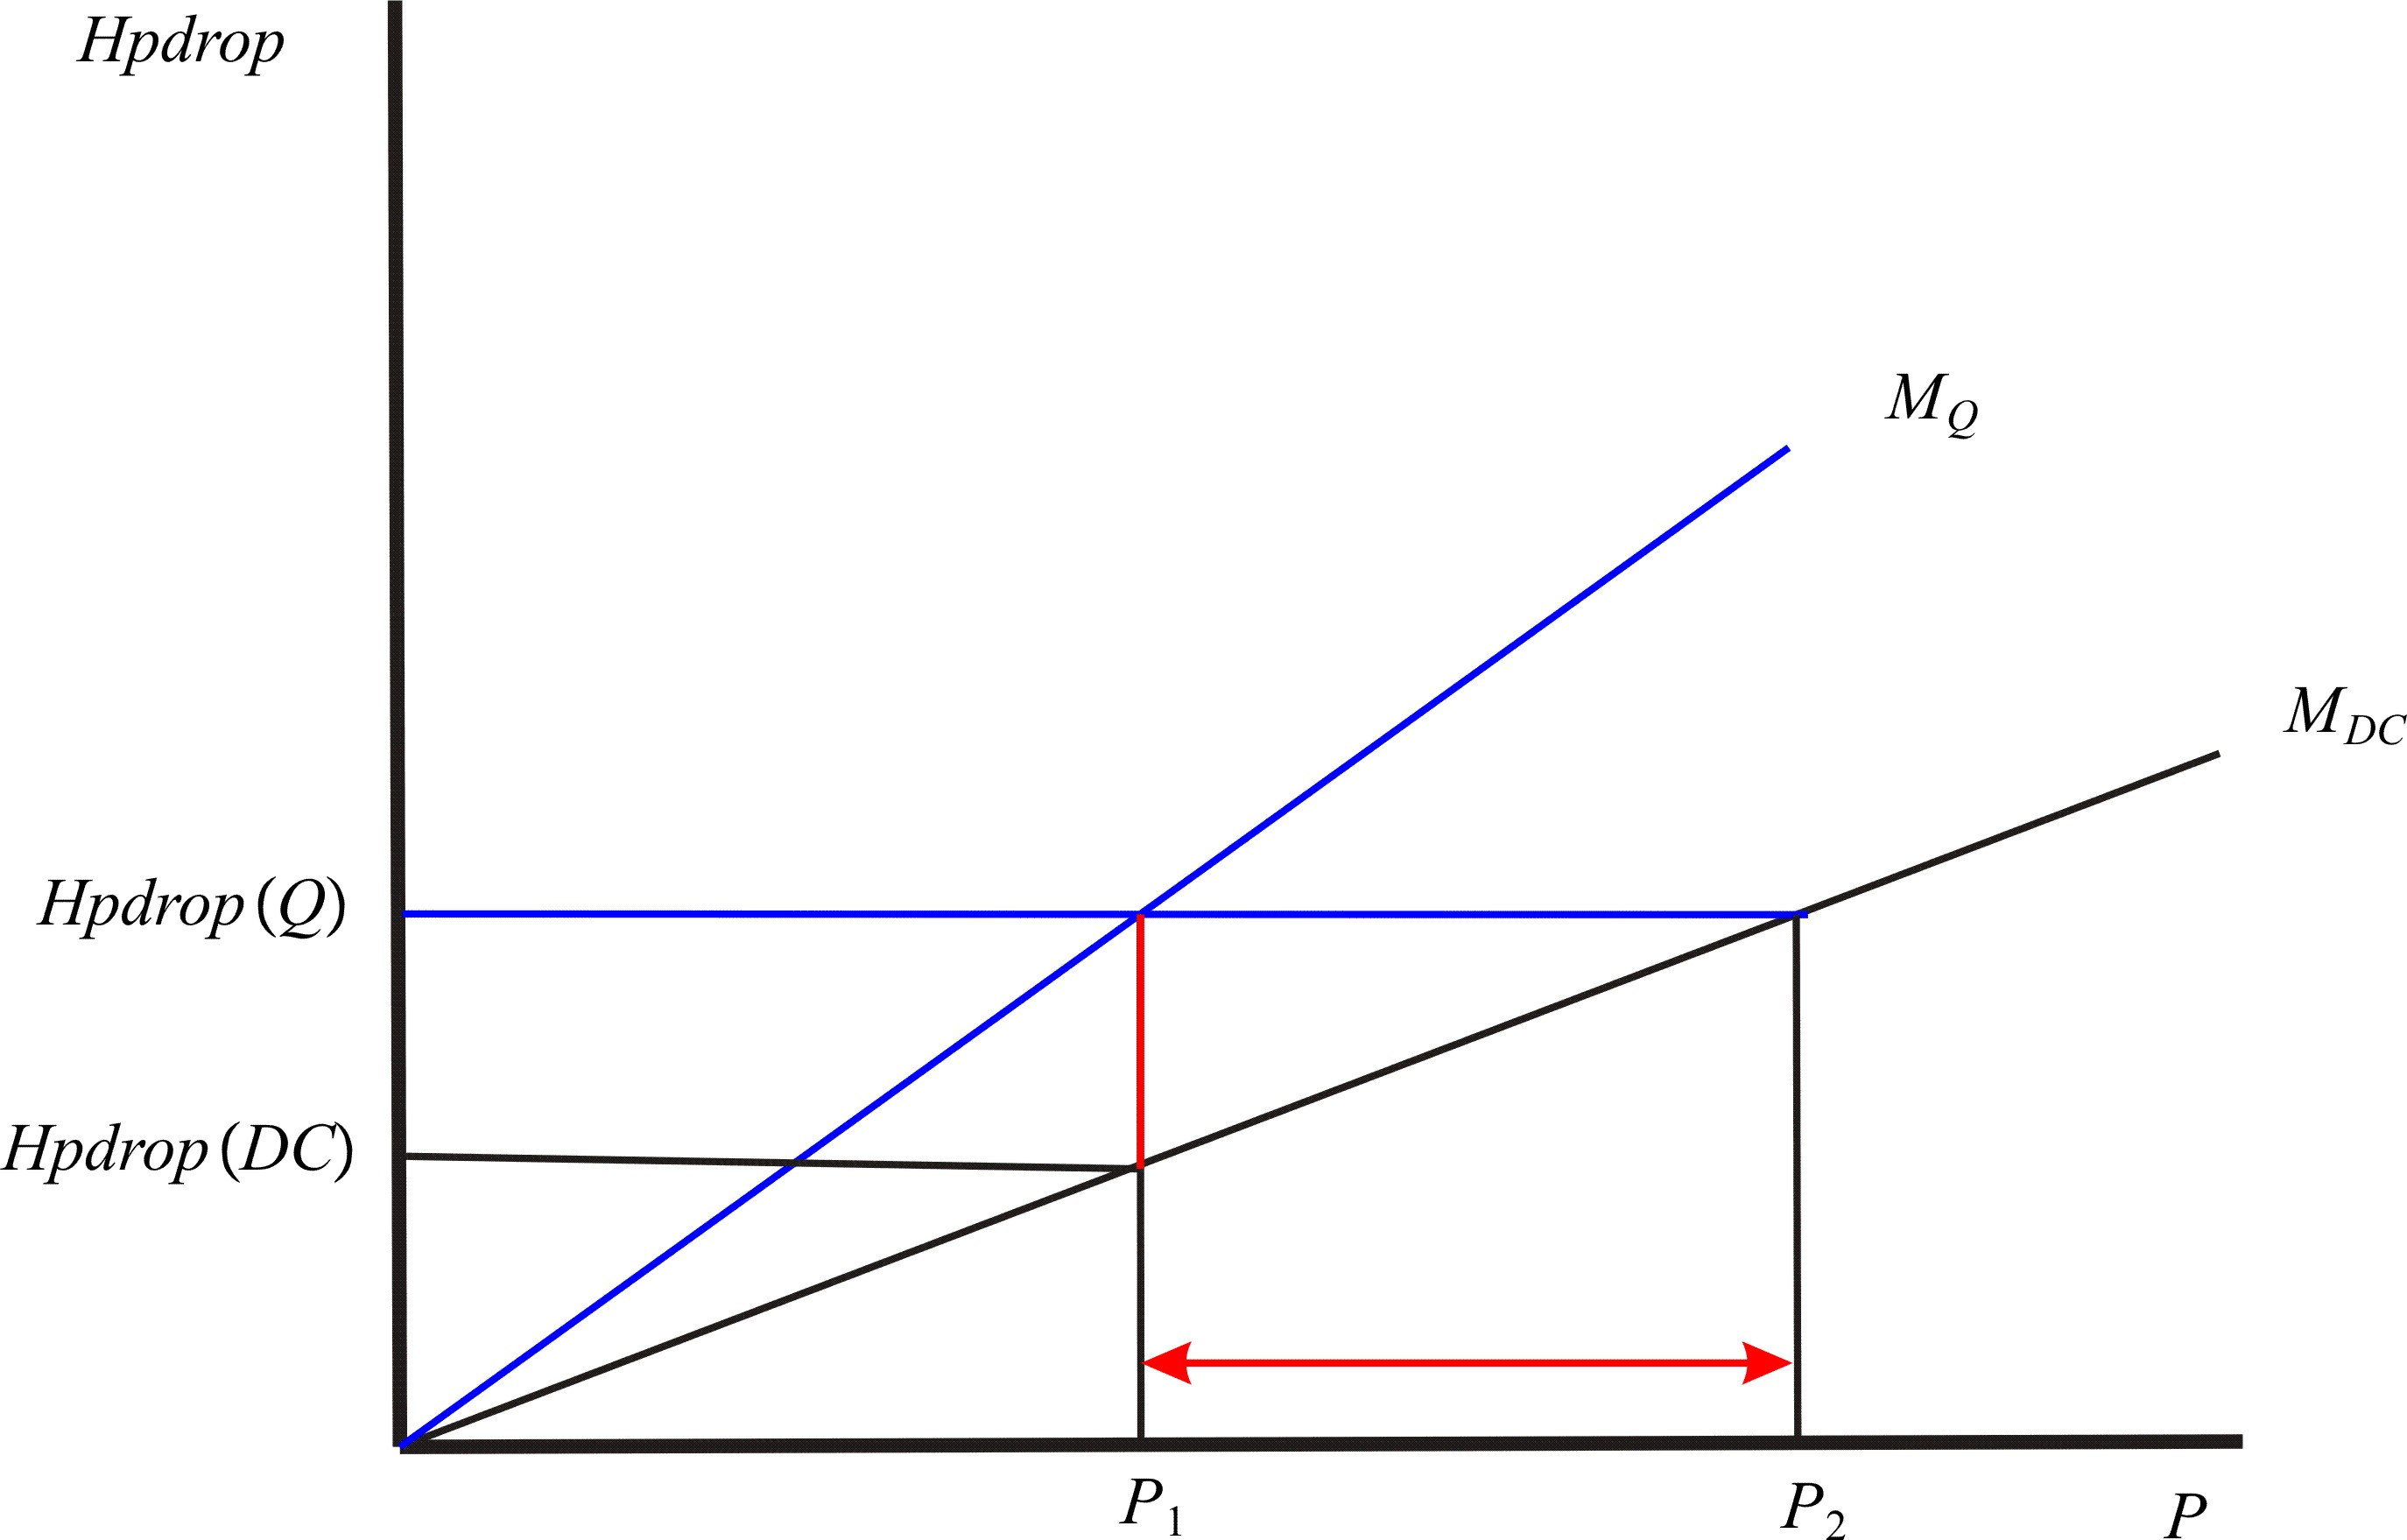
\includegraphics[scale=0.5]{jin1.jpg} 
\caption{Hpdrop vs. P}%
\end{center}
\end{figure}
At a given core temperature\\

Method 1:
\begin{equation}
cop=1+\frac{Hpdrop(Q)-Hpdrop(DC)}{P}= 1+M_{Q}-M_{DC}\ \label{4}%
\end{equation}
Method 2:\\

Assuming $LENR = P_{2}-P_{1}$ see the Figure 1. 
\begin{equation}
cop=1+\frac{LENR}{P_{1}}=1+\frac{Hpdrop(Q)-Hpdrop(DC)}{M_{DC}*P_{1}}= \frac{M_{Q}}{M_{DC}} \ \label{4}%
\end{equation}
\\
COP calculation of ipb1-30b and sri-ipb2-27b based on the method 2, normalized at the temperature 200c, which means at 200c COP = 1, and x axis is the temperature in below Figure 2 and 3. 
\begin{figure}
[h]
%\begin{top}
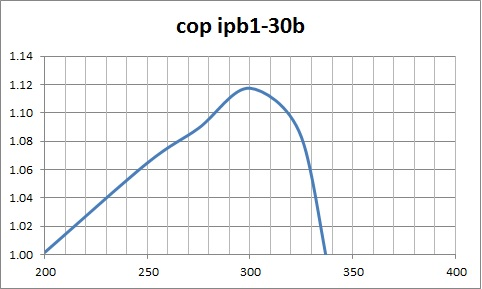
\includegraphics[scale=1.0]{ipb1-30b-cop.jpg} 
\caption{cop vs. temperature of ipb1-30b}%
%\end{top}
\end{figure}

\begin{figure}
%[h]
%\begin{bottom}
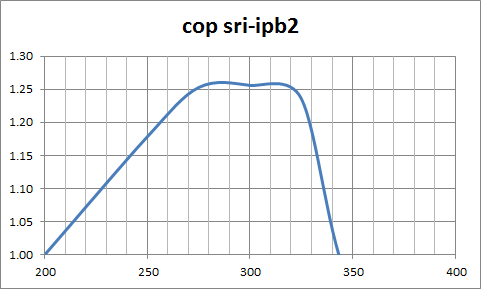
\includegraphics[scale=1.0]{sri-ipb2-27b-cop.png} 
\caption{cop vs. temperature of sri-ipb2-27b}%
%\end{bottom}
\end{figure} 


\end{document}